\documentclass[a4paper, 11pt]{article}
\usepackage{titlesec}
\usepackage{longtable}
\usepackage{listings}
\usepackage{graphicx}
\usepackage[fleqn]{mathtools}
%\titleformat{\subsection}[runin]{\bfseries}{\thesection}{1em}{}[]
%\titleformat{command}[shape]{format}{label}{sep}{before}[after]
\setlength{\mathindent}{0pt}
\lstset{language=C++}
\lstset{breaklines}
\lstset{extendedchars=false}

\title{Experiment Report \\ \begin{large}--- Matrix Multiplication\end{large}}
\author{Name:Wang Xingyi StudentID:5140309531}
\date{\today}

\begin{document}
\maketitle
\section{Introduction}
Given two matrices A and B, where A is a matrix with M rows and K columns and matrix B contains K rows and N columns, the matrix product of A and B is matrix C, where C contains M rows and N columns. The entry in matrix C for row i column j($C_{ij}$) is the sum of the products of the elements for row i in matrix A and column j in matrix B. In this project, the multiplication can be implemented by both single-thread and multi-thread programming. Comparing the running time, we can have a more specific understanding about multi-thread programming.
\section{Running environment}
$\longrightarrow$ Ubuntu 16.04
\section{Experimental procedure}
\subsection{Single-thread programming}
The implementation of matrix multiplication by single-thread programming is quite easy. All we need to do is calculating each element in matrix C separately. The time complexity is $O(n^3)$. The core of the source code is shown below:
\begin{lstlisting}
for(row = 0; row < M; ++row){
    for(column = 0; column < N; ++column){
        multi(row, column);
    }
}
\end{lstlisting}
\subsection{Multi-thread programming}
\subsubsection{Each element in a worker thread}
The method that textbook shows is to calculate each element $C_{ij}$ in a separated worker thread. This will involve creating M $\times$ N worker threads. We use Pthread to do this task. A thread is created by \emph{pthread\_create()}. The arguments are pointed to the function to be executed in each thread and the parameters needed in that function. We define the matrices A, B and C as global variables, so the parameters passed to each thread is the value of row i and column j. So we need a data structure to pass the parameters.
\begin{lstlisting}
typedef struct{
    int row;
    int column;
} matrixWorkInfo;
\end{lstlisting}
After the multiplication, we use \emph{pthread\_join()} to join each thread into the main one.
\begin{lstlisting}
void peer_multi(matrixWorkInfo *workInfo){
    int row = workInfo->row;
    int column = workInfo->column;
    int position;
    C[row][column] = 0;
    for (position = 0; position < K; ++position) {
        C[row][column] = C[row][column] + (A[row][position] * B[position][column]);
    }
    free(workInfo);
}

for (row = 0; row < M; ++row){
    for (column = 0; column < N; ++column){
    	id = N * row + column;
    	workInfo = (matrixWorkInfo *)malloc(sizeof(matrixWorkInfo));
    	workInfo->row = row;
    	workInfo->column = column;
    	pthread_create(&(peer[id]), NULL,(void *)peer_multi, (void *)workInfo);
    }
}

for (i = 0; i < (M * N); ++i){
    pthread_join(peer[i], NULL);
}
\end{lstlisting}
\subsubsection{Each row in a worker thread}
But as the scale of the matrix gets larger, the number of thread is growing fast, too. For example, the multiplication of two 1000 $\times$ 1000 matrices will create 1,000,000 threads, which memory cannot afford. So We can calculate each row of matrix C in a separated worker thread.
\begin{lstlisting}
void peer_multi(int *arg){
    int row = *arg;
    int column, position;
    for (column = 0; column < N; ++column) {
    	C[row][column] = 0;
    	for (position = 0; position < K; ++position) {
    	   C[row][column] = C[row][column] + (A[row][position] * B[position][column]);
    	}
    }
}

for (row = 0; row < M; ++row){
    id = row;
    int *arg = (int *)malloc(sizeof(int));
    *arg = row;
    pthread_create(&(peer[id]), NULL, (void *)peer_multi, arg);
}
for (i = 0; i < M; ++i){
    pthread_join(peer[i], NULL);
}
\end{lstlisting}
\subsection{Note}
\subsubsection{Time calculation}
We use \emph{time{}} function to calculate the executing time instead of \emph{clock()}, because the later one is calculating the CPU executing clocks, which will be wrong when there is multi-thread programming.
\begin{lstlisting}
time_t start, finish;
double duration;
start = time(NULL);
\\calculation
finish = time(NULL);
duration = (double)(finish - start);
\end{lstlisting}
\section{Conclusion and Discussion}
The result of calculating two 1000 $\times$ 1000 matrices is:

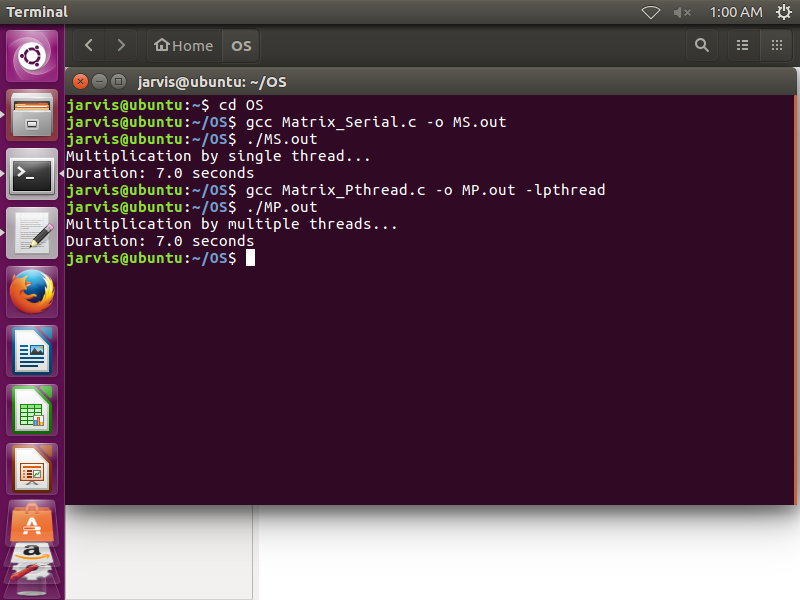
\includegraphics[width=10cm]{pic/1000.png}

The result of calculating two 1500 $\times$ 1500 matrices is:

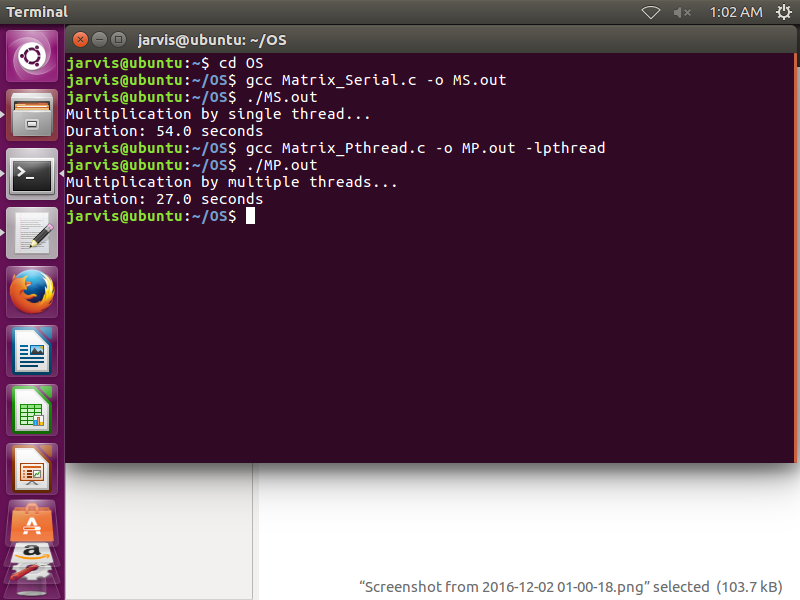
\includegraphics[width=10cm]{pic/1500.png}

The result of calculating two 2000 $\times$ 2000 matrices is:

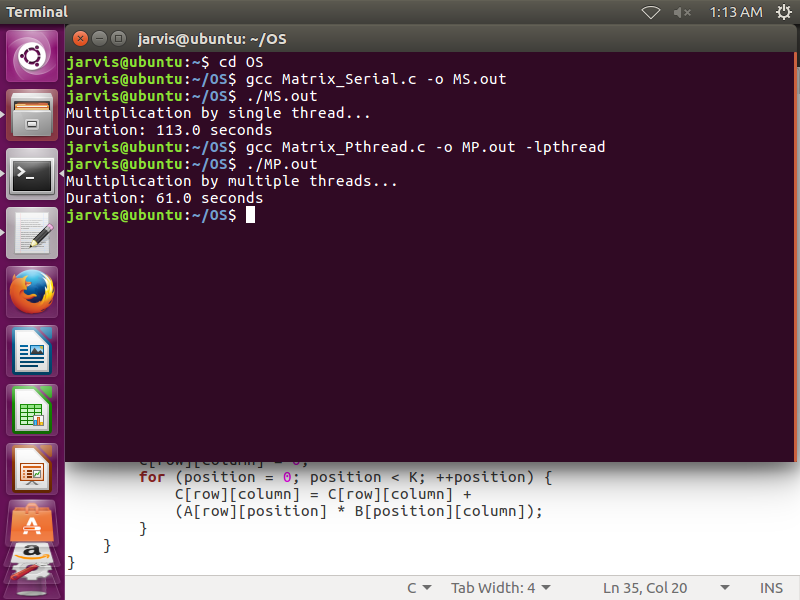
\includegraphics[width=10cm]{pic/2000.png}

It's easy to see that when calculating 1000 $\times$ 1000 matrix multiplication, the executing time is approximately the same. But as the scale of matrices gets larger, the priority of multi-thread programming becomes more obvious. 
\end{document}
